\documentclass[../main.tex]{subfiles}
	% ELECTRONICS TESTING
\begin{document}

Assessing the capabilities of the test bed is split into three main sections.
The first and second sections deal with the electrical and computational characteristics respectively of the Raspberry Pi, and the third deals with the components used in the test bed.
The electrical section pertains to the GPIO pins and their physical capabilities, whereas the computational section considers how fast the pin values can be changed and read by the underlying code, and how most efficiently to achieve this.
The final section discusses limitations to the methods discussed in the above sections, which are posed by the components' specifications.\\

%%%%%%%%%%%%%%%%%%%%%%%%%%%%%%%%%%%%%%%%%%%%%%%%%%%%%%%%%%%%%%%%%%%%%%%%%%%%%%%%%%%%%%%%%%%%%%%%%%%%%%%%%%%%%%%%%%%%%%%%%%%%%%%%%%

\section{Electrical Characteristics of the Raspberry Pi}

The Raspberry Pi 3B has 40 pins, including eight ground pins, two \SI{3.3}{\volt} power pins and two \SI{5}{\volt} power pins.
26 of the remaining pins (BCM pins 2 to 27) are free to be used as General Purpose Input/Output (GPIO).
The GPIO pins can output low (\SI{0}{\volt}) and high (\SI{3.3}{\volt}) levels, and they are powered by the same \SI{3.3}{\volt} rail as the power pins of the same voltage.
As a result, there is a maximum current that can be drawn from all of these pins together as well as from each GPIO pin individually.\\

The Embedded Linux Wiki \cite{web_RpiMaxRatings} claims that the \SI{5}{\volt} pins can provide a maximum current equal to, "The USB [power cable] input current (usually \SI{1}{\ampere}) minus any current draw from the rest of the board."
It also provides the maximum current to be drawn from all \SI{3.3}{\volt} power pins as \SI{50}{\milli\ampere} (this would apply to the power pins and the GPIO pins combined).
However that specification was actually a design value for the original Pi, designed to supply \SI{3}{\milli\ampere} for each of its17 pins for $\approx \SI{51}{\milli\ampere}$ total, according to Gert Van Loo, the hardware engineer of the first Pi's boards \cite{web_RPiSpecsSE}.
There is no current-limiting on the pins so they will attempt to drive the current pulled they stops working, however multiple sources including Gert Van Loo suggest that the maximum current that should be drawn from any one pin for safe operation is \SI{16}{\milli\ampere} as this is the current to which the electronics on each pad are rated.
Mosaic Documentation Web also has a page attempting to define the electrical specifications of the Raspberry Pi \cite{web_MosaicSpecs}, and it also suggests that one shouldn't attempt to source or sink more than \SI{16}{\milli\ampere} on an output pin.
The pins actually have a set drive strength from \SIrange{2}{16}{\milli\ampere} in \SI{2}{\milli\ampere} increments which is set for a bank of pins and usually set to \SI{8}{\milli\ampere} but even a pin set to \SI{2}{\milli\ampere} drive strength and then loaded so as to draw \SI{2}{\milli\ampere} will not be damaged \cite{web_GPIOPadsErrata}.\\

The maximum current which can be drawn from an output pin is a useful detail.
This is both in order to ensure that none of the attached components draw too much current, as well as to decide, along with the input impedances of the pins, whether or not the GPIO pins of one Pi can be connected directly to another without a protective resistor between them.
The input and output impedances of the pins in various set-up modes are investigated in Table \ref{tab_Pin Impedances}.
All values were measured on a multi-meter and using the pin GPIO4 as pins 2 and 3 have permanent internal pull-up resistors whereas all of the rest have software-controllable pull-up or pull-down resistors.\\

\begin{table}[h]
	\centering
	\global\tabulinesep = 2mm
	\begin{tabu} to 0.8\textwidth { | X[l] | X[c] | }
		\hline
		Input/Output Mode & Impedance to Ground ($\SI{}{\kilo\ohm}$)\\
		\hline\hline
		Input & 48.93\\
		\hline
		Input with Pull Up Resistor  & NEED TO DOUBLE CHECK\\
		\hline
		Input with Pull Down Resistor  & NEED TO DOUBLE CHECK\\
		\hline
		Output & NEED TO DOUBLE CHECK\\
		\hline
		Raspberry Pi ON (No Mode) & NEED TO DOUBLE CHECK\\
		\hline
		Raspberry Pi OFF & 53 550\\
		\hline
	\end{tabu}
	\caption{Table of GPIO Pin Impedances for Different Operating Modes}
	\label{tab_Pin Impedances}
\end{table}

These impedances show that even the lowest input impedance of \SI{48.93}{\kilo\ohm} will only draw \SI{67.44}{\micro\ampere} of current from a \SI{3.3}{\volt} GPIO pin, three orders of magnitude lower than the maximum current enough that these pins from one Raspberry Pi can be connected directly to those of another. 
The ground pins of Raspberry Pis must be connected together so that they share a common reference for the data levels.\\

\clearpage

%%%%%%%%%%%%%%%%%%%%%%%%%%%%%%%%%%%%%%%%%%%%%%%%%%%%%%%%%%%%%%%%%%%%%%%%%%%%%%%%%%%%%%%%%%%%%%%%%%%%%%%%%%%%%%%%%%%%%%%%%%%%%%%%%%

\section{Computational Characteristics of the Raspberry Pi} \label{sec_Computation}

\todo[inline,color=blue!20]{Write Computing and Components Sections - I have all the data, screen shots and component characterising values}

time.time() in for loop - 3.32 us
time.time() in while loop with i++ - 4.02 us = slower
time.time() sequential - 2.81 us
therefore for loop time - 0.51us

100Hz (excluding the 10ms)
sleep(1/freq) - 104.13 us
sleep(1/freq-timeDif) - 90.08 us == REMOVES DELAY OF ~15us - GPIO AND A BIT
SAME without sleep(1/freq) (just GPIO) - 5.18 us
SAME without GPIO.output (just sleep(1/freq)) - 97.18 us == SLEEP IS THE INEFFICIENT FUNCTION LOSING ME TIME
You can hard-code in the ~104e-6 value to get offset of ~5us instead of 104us but this is not ideal - need to compare to coding in c...\\

Table from interim report and two screen shots in particular.\\

\begin{figure}[ht]
	\centering
	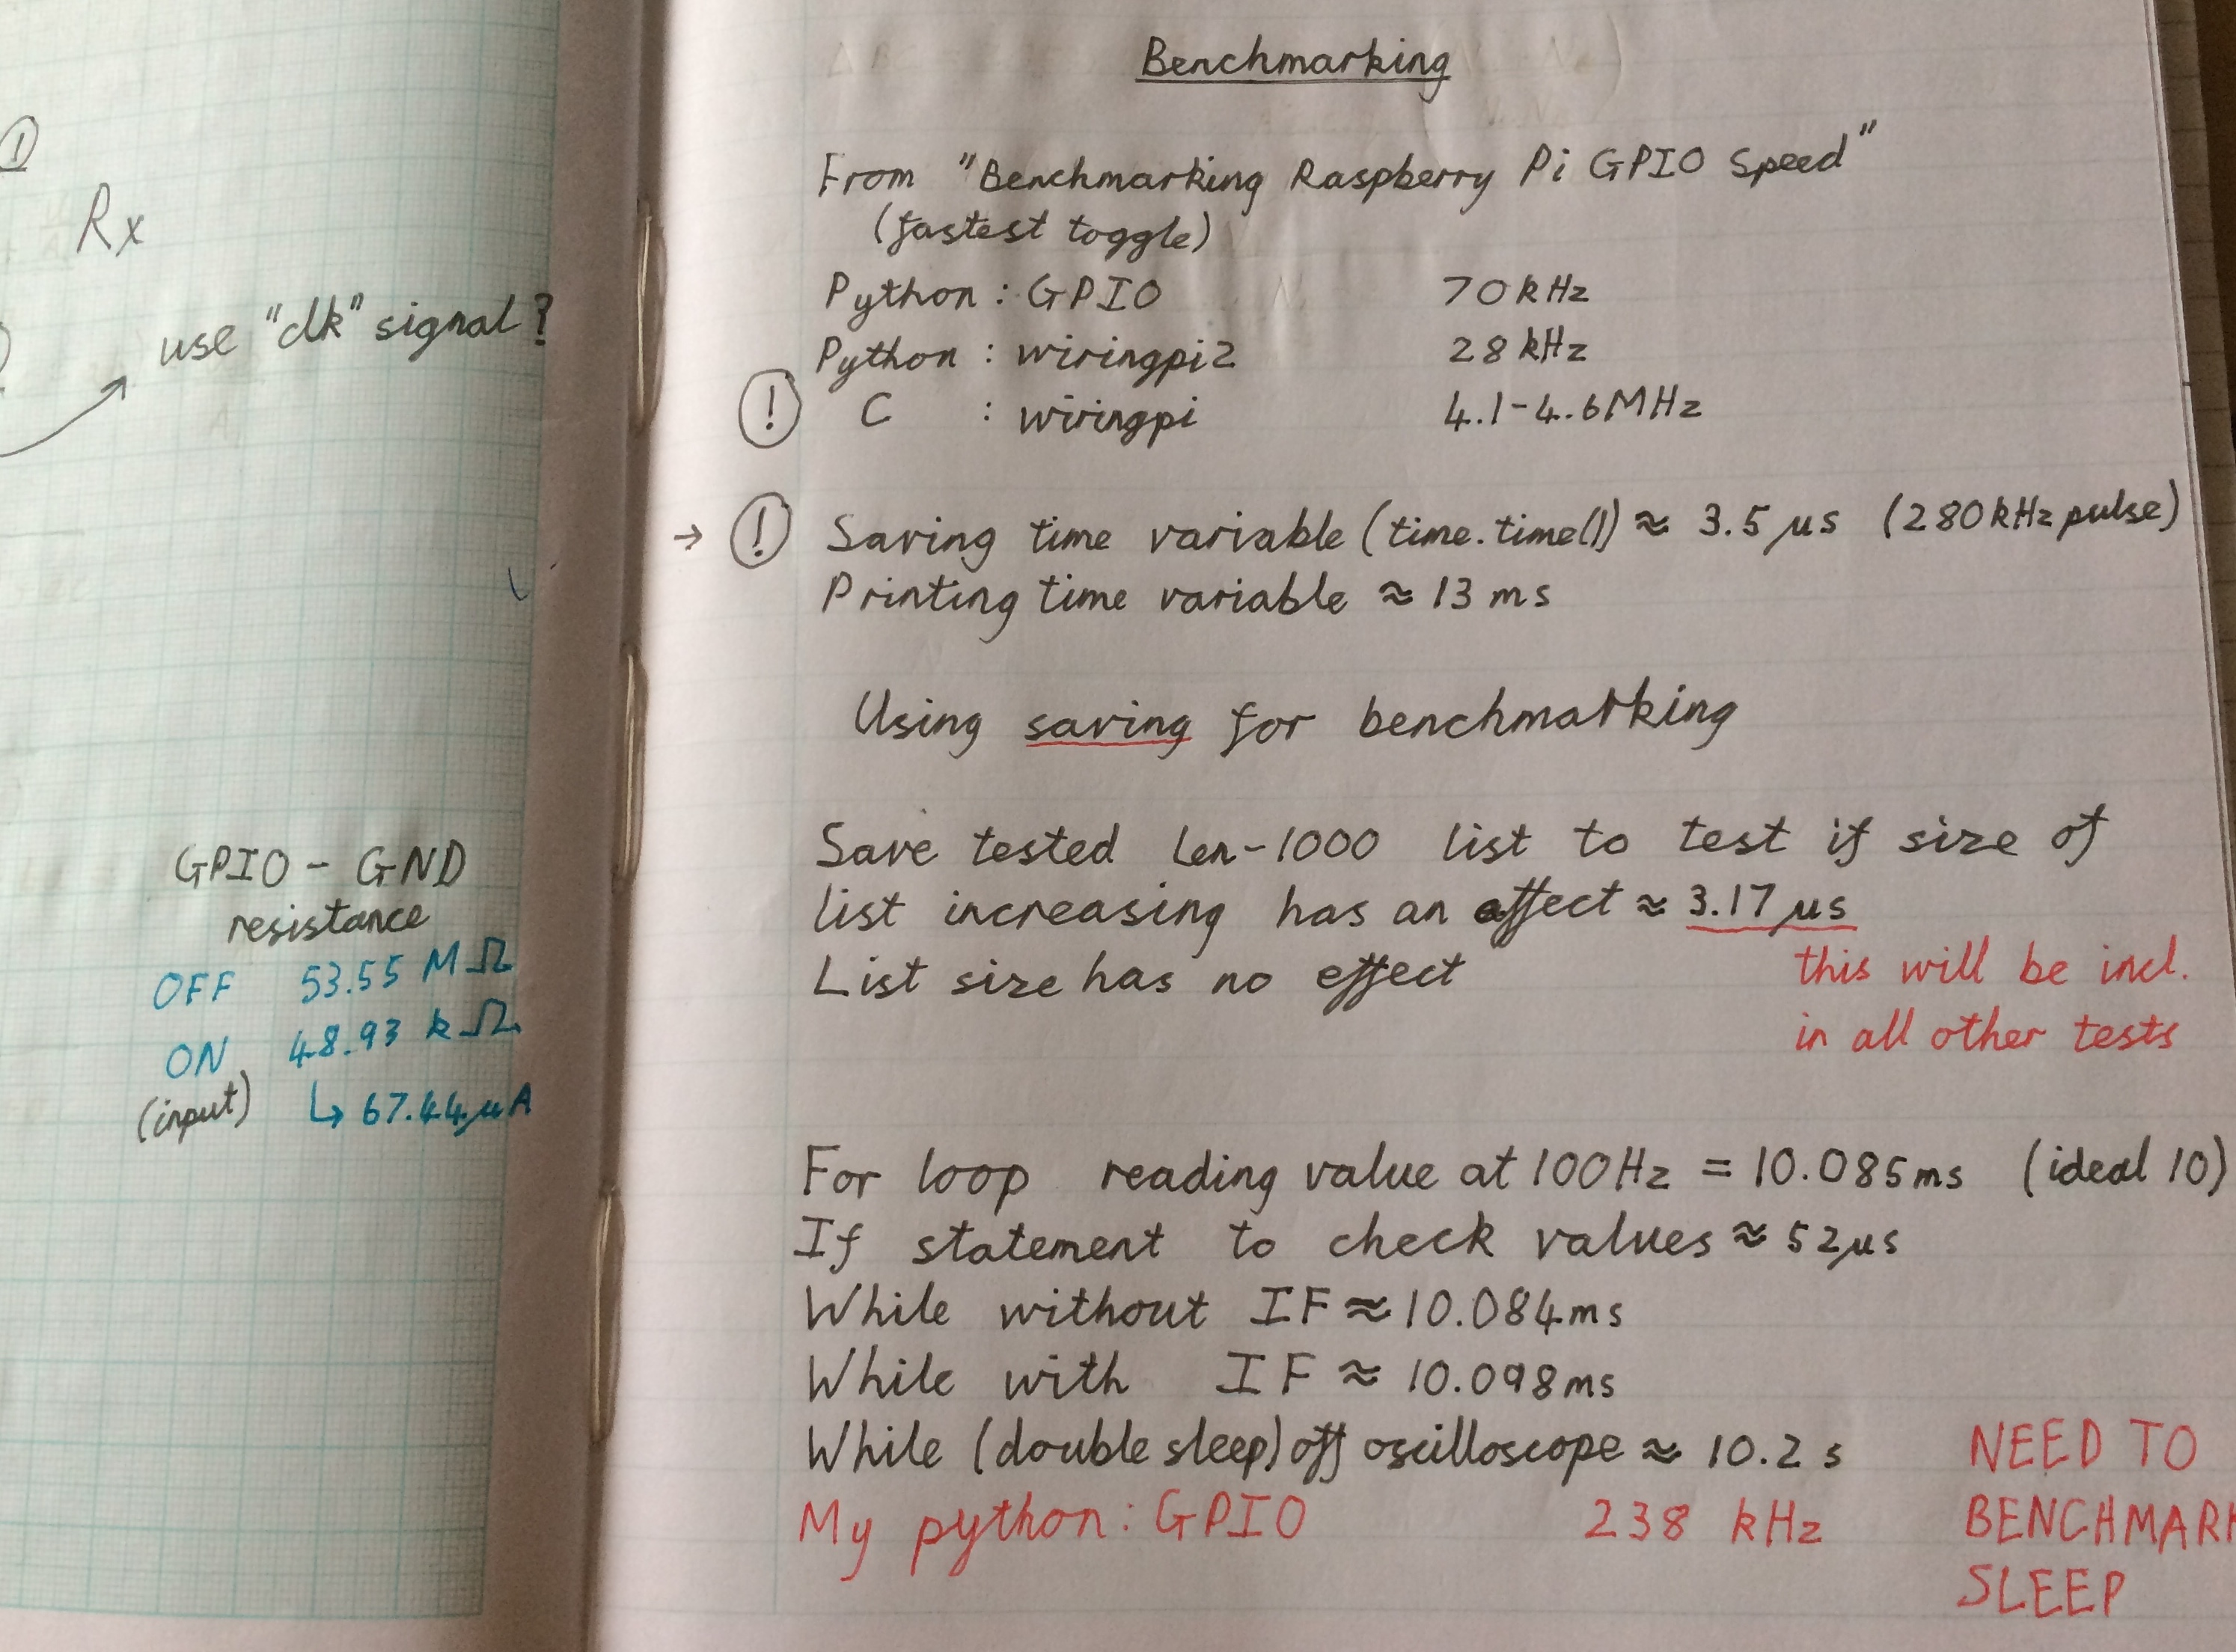
\includegraphics[width=0.6\textwidth]{Benchmarking_Data.jpg}
	\caption{Benchmarking initial data collection}
	%\label{fig_}
\end{figure}

\subsection{Maximum Frequency}

\todo[inline,color=blue!20]{Comparison of transmitter bank vs individual write and receiver read (callback) and read vars on clock pulse vs bank read on clock pulse -- Also mention }

\subsection{Comparing Python and C} \label{sec_Comparing Python and C}

\clearpage

%%%%%%%%%%%%%%%%%%%%%%%%%%%%%%%%%%%%%%%%%%%%%%%%%%%%%%%%%%%%%%%%%%%%%%%%%%%%%%%%%%%%%%%%%%%%%%%%%%%%%%%%%%%%%%%%%%%%%%%%%%%%%%%%%%

\section{Characterising Components of the Test Bed} \label{sec_Components}

\begin{figure}[ht]
	\centering
	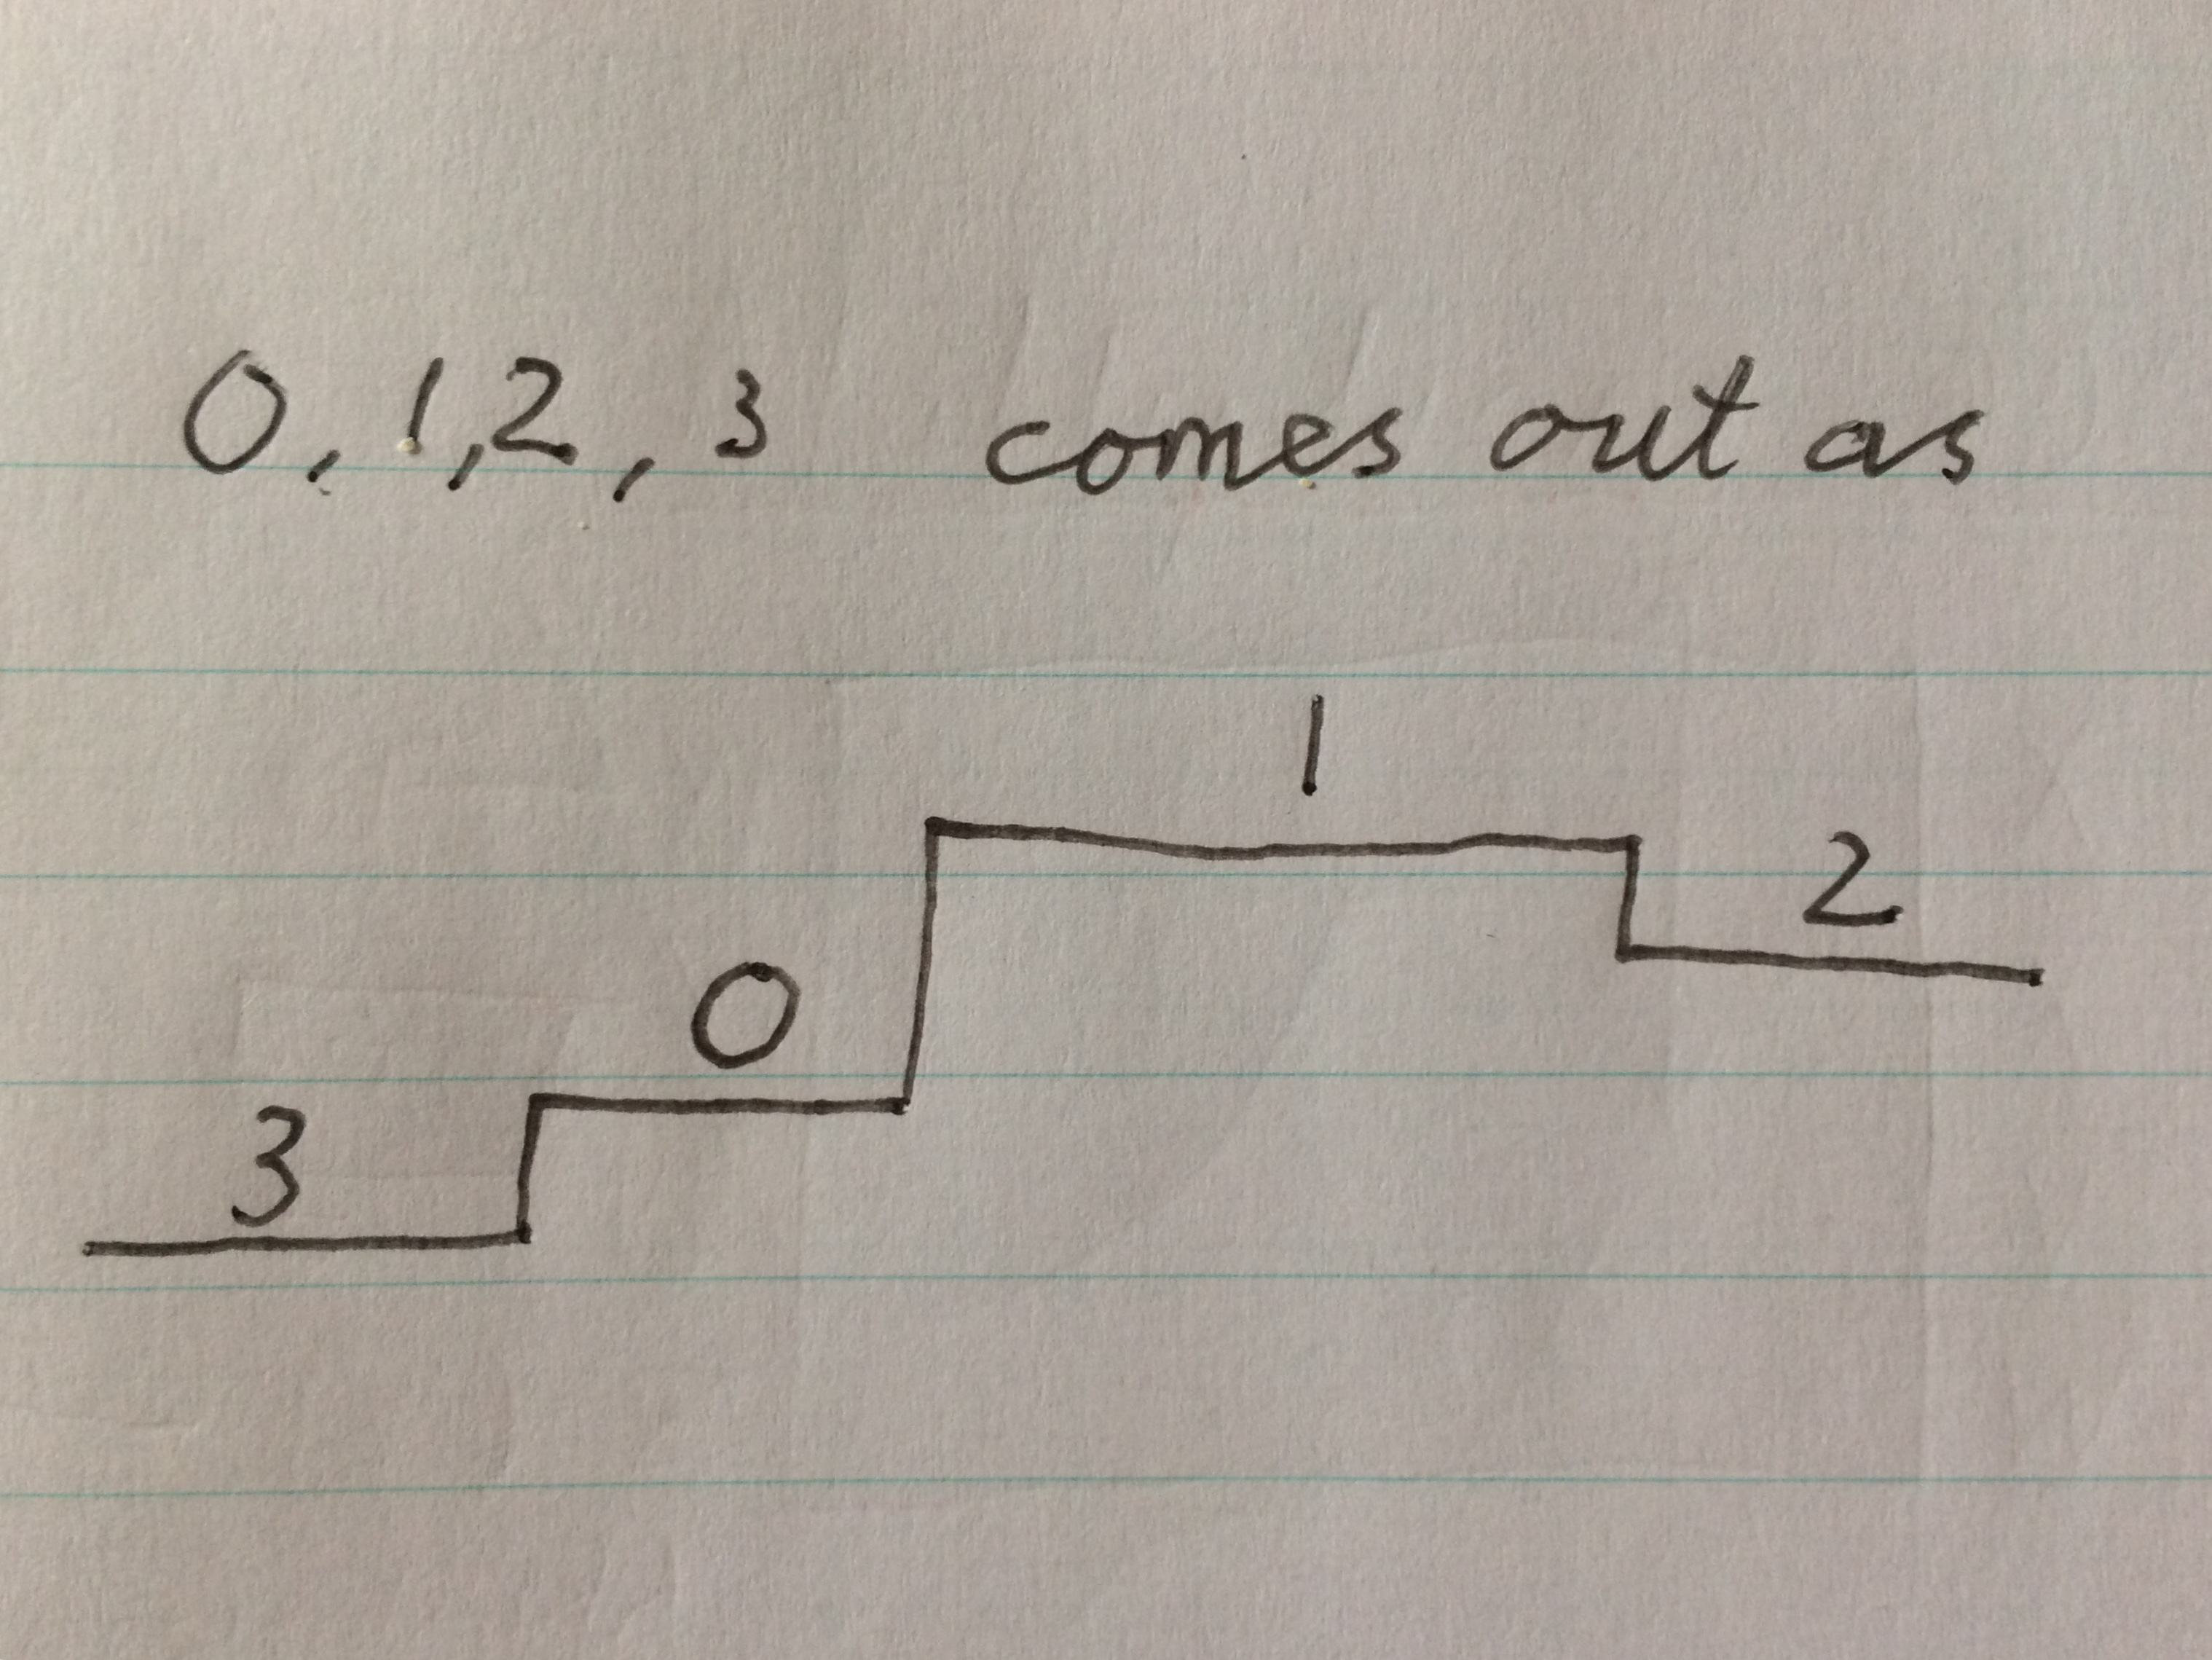
\includegraphics[width=0.4\textwidth]{DAC_Output.jpg}
	\caption{Non-continuous Output for Continuous Input Values of the DAC}
	%\label{fig_}
\end{figure}

\begin{figure}[ht]
	\centering
	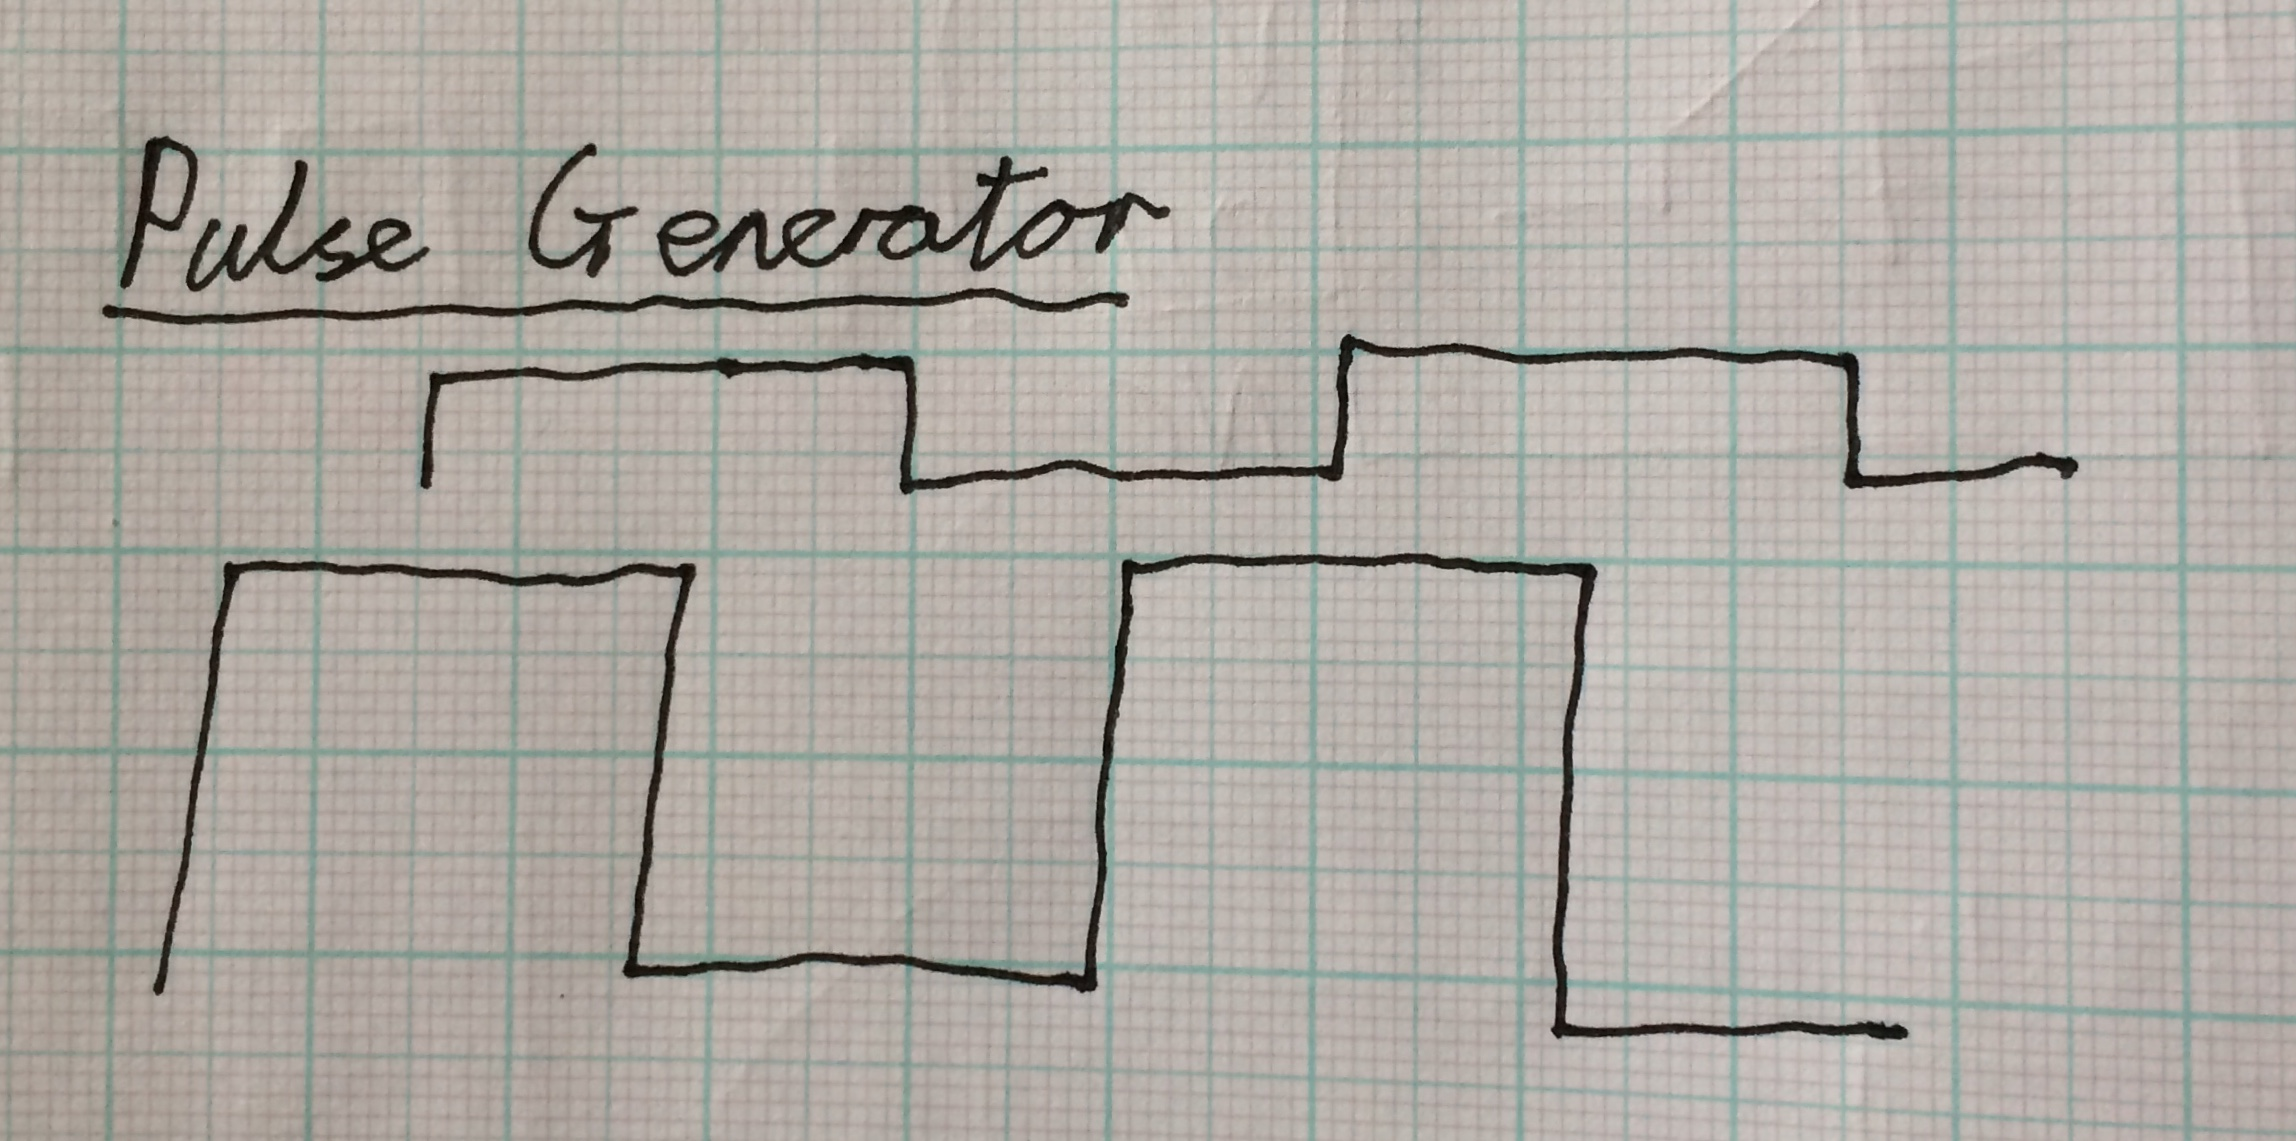
\includegraphics[width=0.6\textwidth]{Pulse_Output.jpg}
	\caption{Output of pulse generator}
	%\label{fig_}
\end{figure}

\begin{figure}[ht]
	\centering
	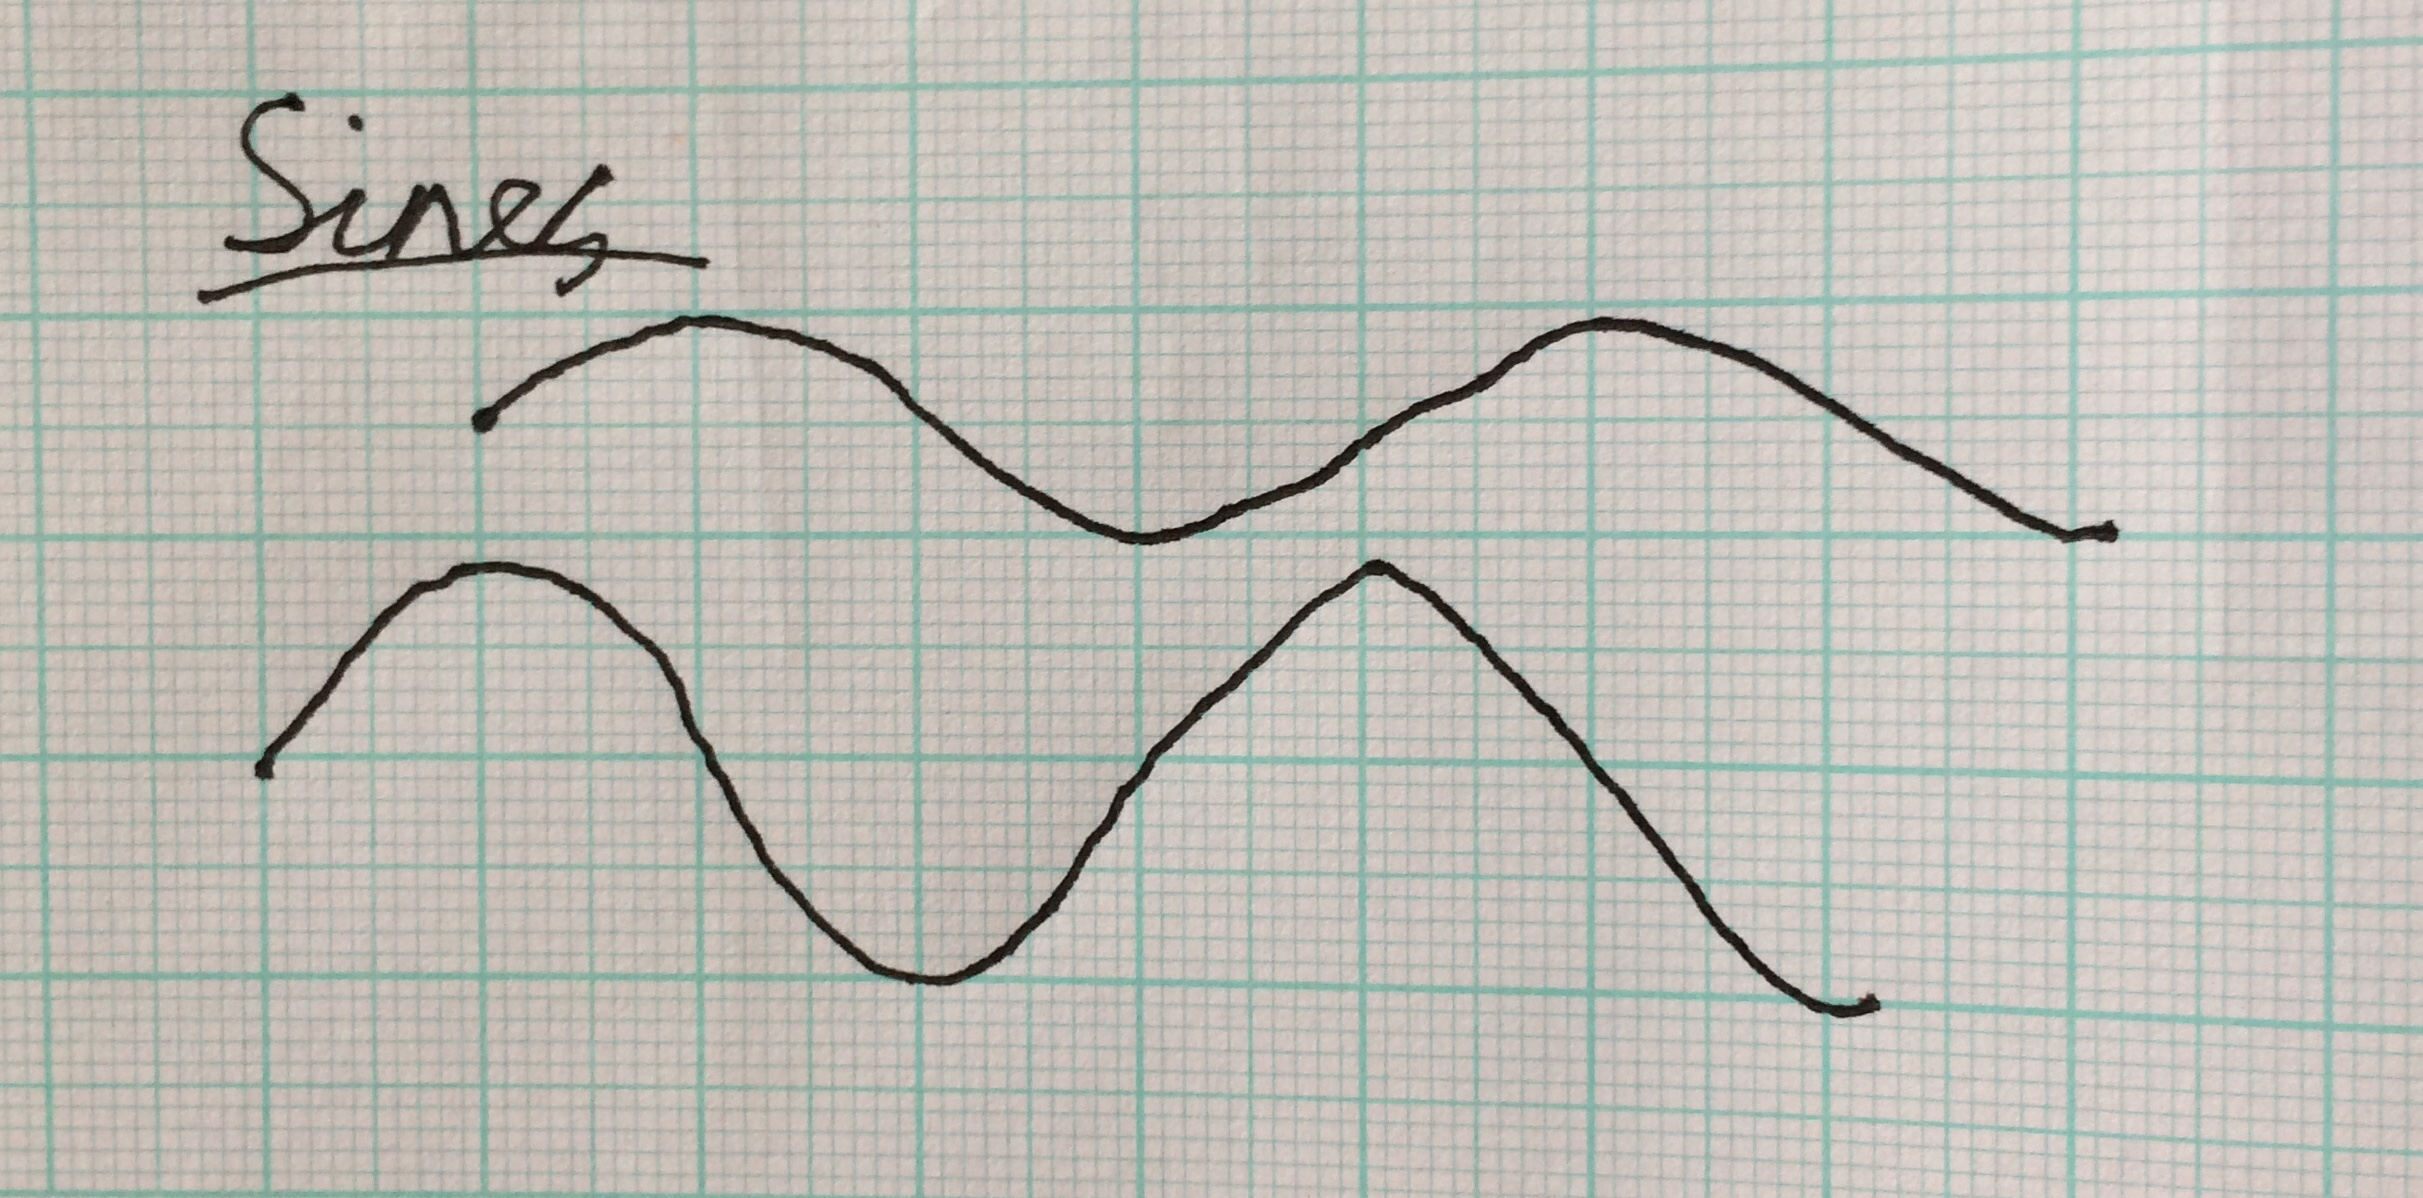
\includegraphics[width=0.6\textwidth]{Sine_Output.jpg}
	\caption{Output of pulse generator once filtered to be sine waves}
	%\label{fig_}
\end{figure}



Electrical Components:
\begin{itemize}
	\item Analogue Digital Converter
	\item Digital Analogue Converter
	\item Quadrature Sinusoid Generator
	\item Multiplier/Mixer
	\item Low Pass Filters
\end{itemize}

\subsection{Overclocking Components}

The \textit{pigpio} library has access to the hardware clocks of the Raspberry Pi.
Specifically on the Pis used, it has the ability to set a hardware clock which is not reserved for system use to a specified frequency between \SI{4.7}{\kilo\hertz} and \SI{250}{\mega\hertz} on pin 4, although the library documentation suggests that frequencies above \SI{30}{\mega\hertz} are unlikely to work \cite{lib_pigpioHWClock}.\\

There are certain components such as the Analogue Digital Converter and the pulse generator which work using an internal clock set by an external resistor, but which may be overclocked by an external clocking signal, and this functionality may be used.
This would allow the frequencies of these devices to be defined in software with less reliance on external physical components.
The pulse generator isn't as good an example as it still uses external filtering to generate sinusoidal outputs, but this is particularly relevant for the ADC as it requires eight clock pulses per conversion, and setting a hardware clock for (at least) eight times the transmission frequency is one way of ensuring this in software.\\

\begin{figure}[ht]
	\centering
	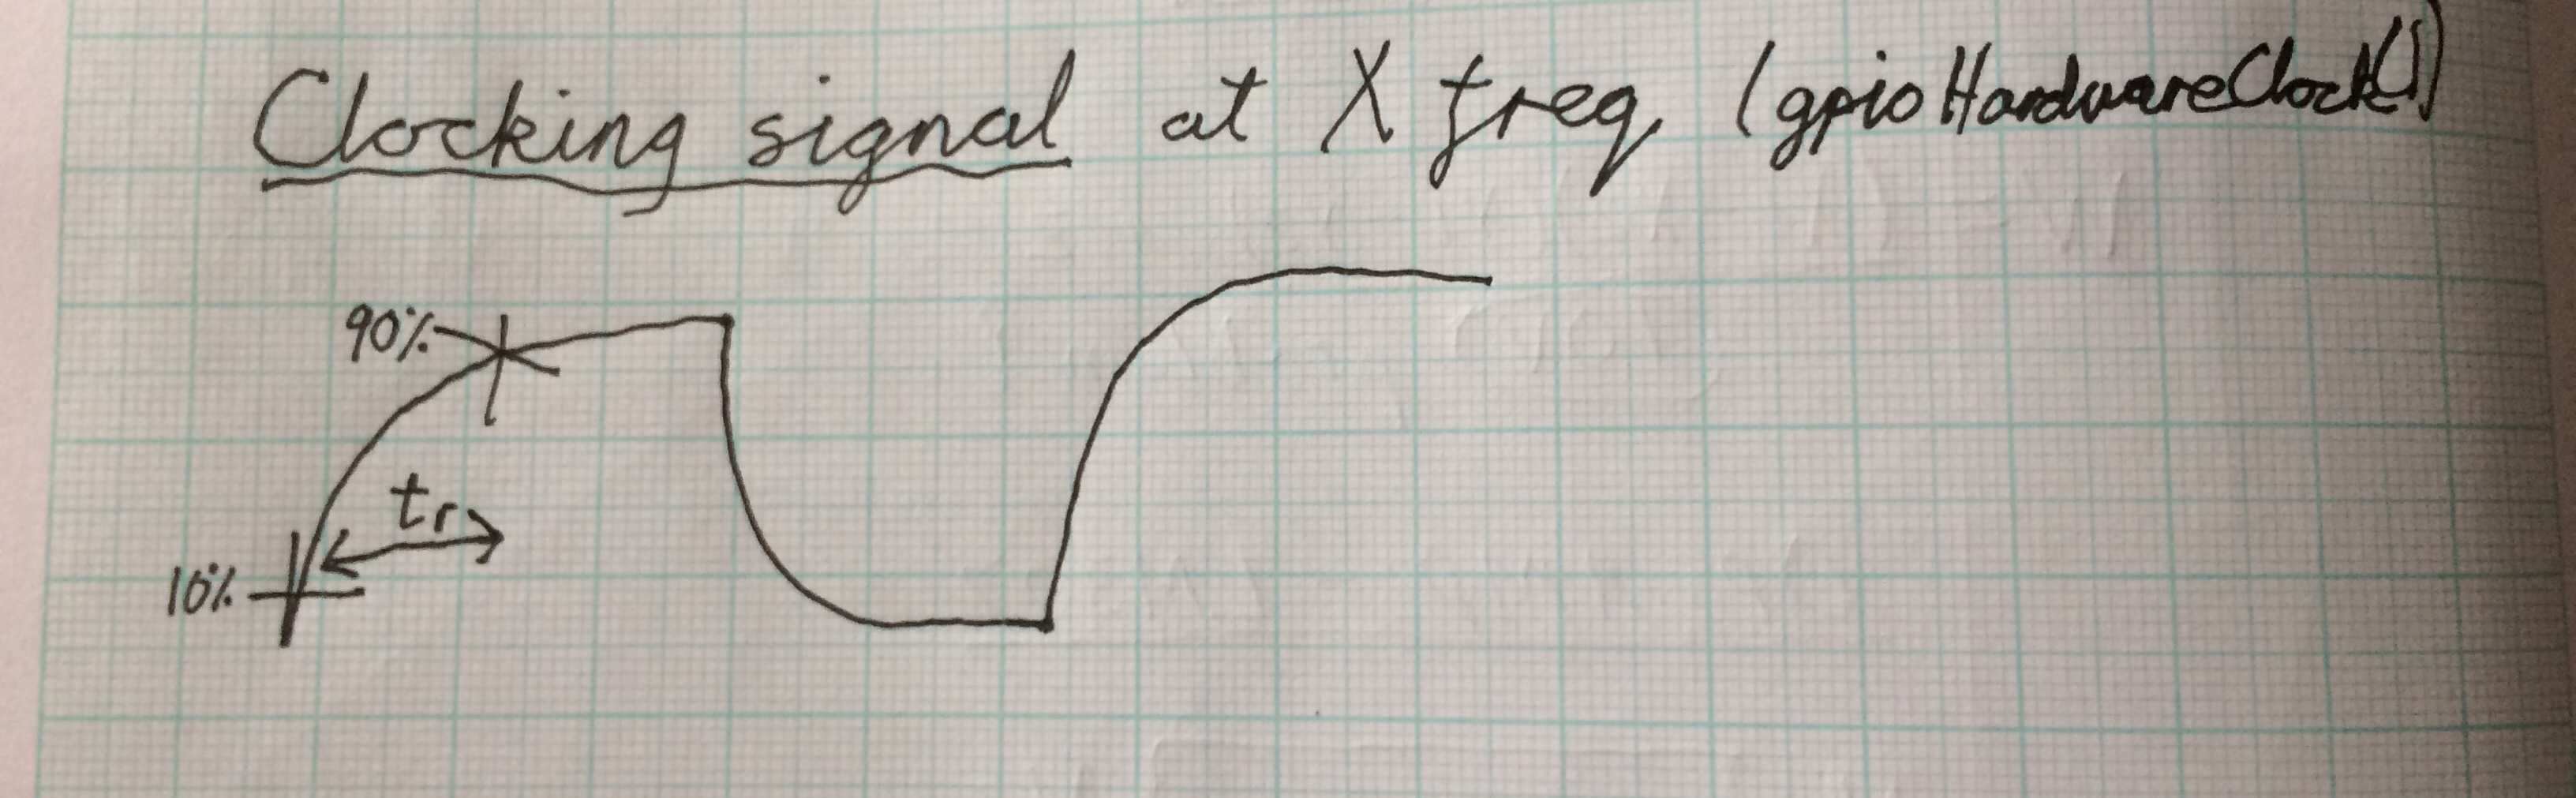
\includegraphics[width=0.6\textwidth]{Clock_Analyse.jpg}
	\caption{This is a high frequency view of the hardware clock for interest and rise-time (max frequency achievable actually) - will analyse screen grab from Oscilloscope and include in report}
	%\label{fig_}
\end{figure}


\end{document}